\documentclass[titlepage=firstiscover, bibliography=totoc, captions=tableheading]{scrartcl}
\author{Felix Geyer \\
  \texorpdfstring{\href{mailto:felix.geyer@tu-dortmund.de}{felix.geyer@tu-dortmund.de}\and}{,}
  Rune Dominik \\
  \texorpdfstring{\href{mailto:rune.dominik@tu-dortmund.de}{rune.dominik@tu-dortmund.de}}{}
  }
\title{V354: Gedämpfte und erzwungene Schwingungen}
\date{Durchführung: 10. Januar 2017 \\
      Abgabe: 17. Januar 2017}
\usepackage[aux]{rerunfilecheck}
\usepackage{polyglossia}
\setmainlanguage{german}
\usepackage{amsmath}
\usepackage{amssymb}
\usepackage{mathtools}
\usepackage{fontspec}

\usepackage{scrhack}
\usepackage{float}
\floatplacement{table}{htbp}
\floatplacement{figure}{htbp}

\usepackage[locale=DE, separate-uncertainty=true, per-mode=symbol-or-fraction, decimalsymbol=.]{siunitx}
%\usepackage{siunitx}

\usepackage[style=alphabetic]{biblatex}
\addbibresource{lit.bib}

\usepackage[section, below]{placeins}
\usepackage[labelfont=bf,
font=small,
width=0.9\textwidth,
format=plain,
indention=1em]{caption}
\usepackage{graphicx}
\usepackage{grffile}
\usepackage{subcaption}

\usepackage[math-style=ISO, bold-style=ISO, sans-style=italic, nabla=upright, partial=upright]{unicode-math}
\setmathfont{Latin Modern Math}

\usepackage[autostyle]{csquotes}

\usepackage[unicode]{hyperref}

\usepackage{bookmark}

\usepackage{booktabs}

\begin{document}

  \section{Auswertung}
  \subsection{Rechteckiger Stab, einseitige Einspannung}
  \begin{table}
    \centering
    \caption{Rechteckiger Stab, einseitige Einspannung}
    \label{tab:data2}
    \begin{tabular}{c c c  }
      \toprule $x \, \,  in \,\, m$ & $D(x) \,\, in \,\,  m$ & $Lx^2-\frac{1}{3}x^3$\\
      \midrule
      0.03 & 0.00780 & 0.0005346\\
      0.05 & 0.00744 & 0.0014683\\
      0.10 & 0.00641 & 0.0057067\\
      0.15 & 0.00525 & 0.0124650\\
      0.20 & 0.00491 & 0.0214933\\
      0.25 & 0.00254 & 0.0325417\\
      0.30 & 0.00120 & 0.0453600\\
      0.35 & 0.00088 & 0.0596983\\
      \bottomrule
    \end{tabular}
  \end{table}
  Die Ausmessung des Stabes und die Masse des Gewichts ergeben:
  \begin{align}
    L &= (0,604 \pm 0,002) \, \mathrm{m} & B &= (1,00 \pm 0,04) \, \mathrm{cm} \\
    m &= 0,1672 \, \mathrm{Kg} \label{eqn:2}
  \end{align}
Für die Ausgleichsgerade in Abbildung \ref{fig:1} ergeben sich die Parameter

\begin{align*}
  a &= (0,183 \pm 0,015) \, \mathrm{\frac{1}{m^2}}
  & b &= (-0,0082 \pm 0,0032) \, \mathrm{m}
\end{align*}
\begin{figure}
  \centering
  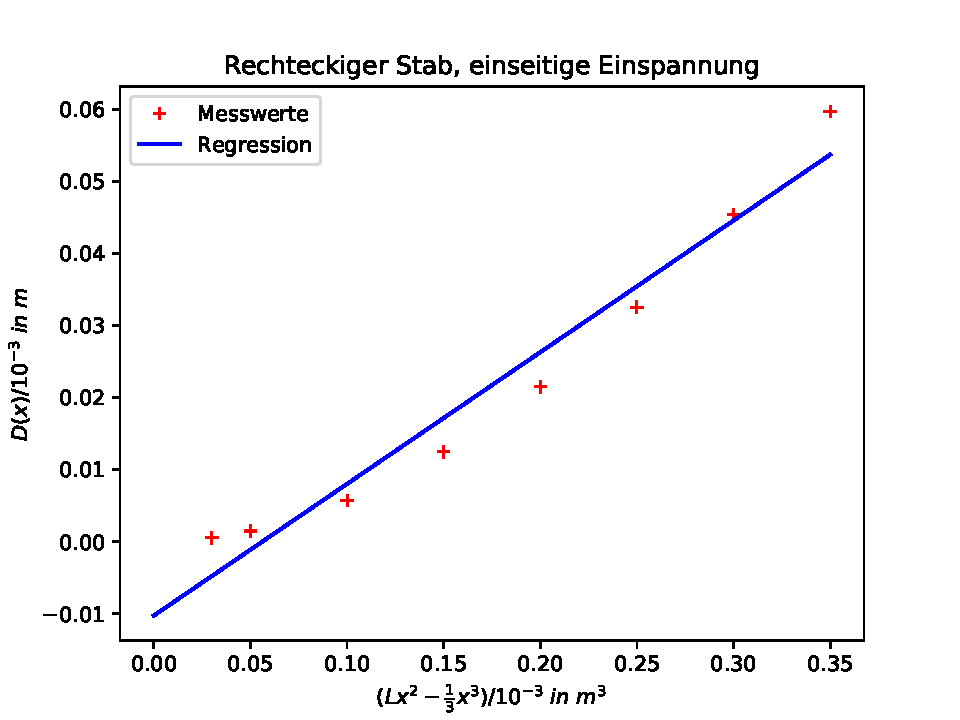
\includegraphics[width=\textwidth]{plot1.pdf}
  \caption{Rechteckiger Stab, einseitige Einspannung}
  \label{fig:1}
\end{figure}
\\
\\
Mit Hilfe der Formel
\begin{equation*}
  I = \frac{ab^3}{12}= \frac{B^4}{12}
\end{equation*}
lässt sich nun das Flächenträgheitsmoment berechnen.
\begin{equation*}
  I = (8,33 \pm 1,33) \cdot 10^{-10} \, \mathrm{m^4}
\end{equation*}
Daraus folgt das Elastizitätsmodul, dass mit der Formel
\begin{equation}
  E = \frac{m\cdot g}{2\cdot a\cdot I}
  \label{eqn:elasti}
\end{equation}
berechnet wird.
\begin{equation*}
  E_{Rechteck}= (53,80 \pm 9,66)\cdot 10^8 \, \mathrm{\frac{N}{m^2}}
\end{equation*}
\newpage
\subsection{Zylindrischer Stab, einseitige Einspannung}
\begin{table}
  \centering
  \caption{Zylindrischer Stab, einseitige Einspannung}
  \label{tab:data2}
  \begin{tabular}{c c c  }
    \toprule $x \, \,  in \,\, m$ & $D(x) \,\, in \,\,  m$ & $Lx^2-\frac{1}{3}x^3$ \\
    \midrule
    0.03 & 0.00800 & 0.0005328\\
    0.05 & 0.00757 & 0.0014633\\
    0.10 & 0.00640 & 0.0056867\\
    0.15 & 0.00506 & 0.0124200\\
    0.20 & 0.00342 & 0.0214133\\
    0.25 & 0.00151 & 0.0324167\\
    0.30 & 0.00080 & 0.0451800\\
    \bottomrule
  \end{tabular}
\end{table}
\begin{figure}
  \centering
  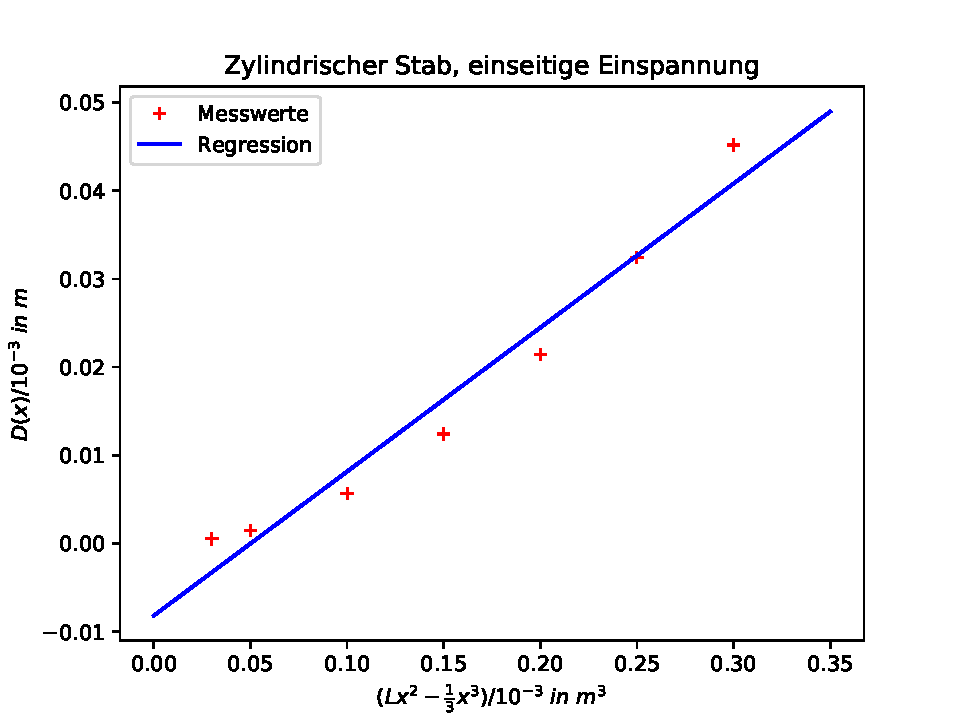
\includegraphics[width=\textwidth]{plot2.pdf}
  \caption{Zylindrischer Stab, einseitige Einspannung}
  \label{fig:2}
\end{figure}
Die gemessenen Werte für die Stablänge $L$,
die Breite $B$ und  die Masse des Stabes lauten:
\begin{align}
  L &= (0,602 \pm 0,002)\, \mathrm{m} & B &= (0,98 \pm 0,03) \, \mathrm{cm} \\
  m &= 0,3954 \, \mathrm{Kg} \label{eqn:9}
\end{align}

Für die Ausgleichsgerade aus Abbildung \ref{fig:2} ergeben sich die Parameter
\begin{align*}
  a &= (0,163 \pm 0,015) \, \mathrm{\frac{1}{m^2}} & b &= (-0,0082 \pm 0,0027) \, \mathrm{m}
\end{align*}

Zur Bestimmung des Flächenträgheitsmoments wird die Formel
\begin{equation*}
  I_{Zylinder} =  \frac{\pi r^4}{4}
\end{equation*}
verwendet. Das führt zu einem Flächenträgheitsmoment von
\begin{equation*}
  I_{Zyl.} = (4,528 \pm 1,109)\cdot 10^{-10} \, \mathrm{m^4}
\end{equation*}
Das Elastizitätsmodul wird mit Formel \ref{eqn:elasti} bestimmt und lautet:
\begin{equation*}
  E_{Zyl.} = (26,28 \pm 6,87) \cdot 10^9 \, \mathrm{\frac{N}{m^2}}
\end{equation*}
\newpage
\subsection{Zylindrischer Stab, beidseitige Einspannung}
\begin{table}
  \centering
  \caption{Zylindrischer Stab, beidseitige Einspannung}
  \label{tab:data2}
  \begin{tabular}{c c c  }
    \toprule $x \, \,  in \,\, m$ & $D(x) \,\, in \,\,  m$ & $3L^2x-4x^3$ \\
    \midrule
    0.03 & 0.00842 & 0.032508\\
    0.05 & 0.00836 & 0.053861\\
    0.10 & 0.00816 & 0.104721\\
    0.15 & 0.00804 & 0.149582\\
    0.20 & 0.00790 & 0.185443\\
    0.25 & 0.00775 & 0.209303\\
    \bottomrule
  \end{tabular}
\end{table}
\begin{table}
  \centering
  \caption{Zylindrischer Stab, beidseitige Einspannung}
  \label{tab:data2}
  \begin{tabular}{c c c  }
    \toprule $x \, \,  in \,\, m$ & $D(x) \,\, in \,\,  m$ & $4x^3-12Lx^2+9Lx-L^3$ \\
    \midrule
    0.30 & 0.00684 & 0.218164\\
    0.35 & 0.00700 & 0.209965\\
    0.40 & 0.00716 & 0.186647\\
    0.45 & 0.00735 & 0.151209\\
    0.50 & 0.00765 & 0.106651\\
    0.55 & 0.00800 & 0.055973\\
    \bottomrule
  \end{tabular}
\end{table}
Hier werden zwei Ausgleichsgeraden bestimmt, da mit zwei Messuhren gemessen wurde.
Dies erfolgt durch eine rechtsseitige Betrachtung und eine linksseitige Betrachtung.
So ergeben sich mittels Python die Paramerter
\begin{align*}
  a_1 &= (0,82 \pm 0,05) \, \mathrm{\frac{1}{m^2}} & b_1 &= (0,016 \pm 0,008) \, \mathrm{m} \\
  a_2 &= (-0,65 \pm 0,08) \, \mathrm{\frac{1}{m^2}} & b_2 &= (0,428 \pm 0,033) \, \mathrm{m}
\end{align*}
\begin{figure}
  \centering
  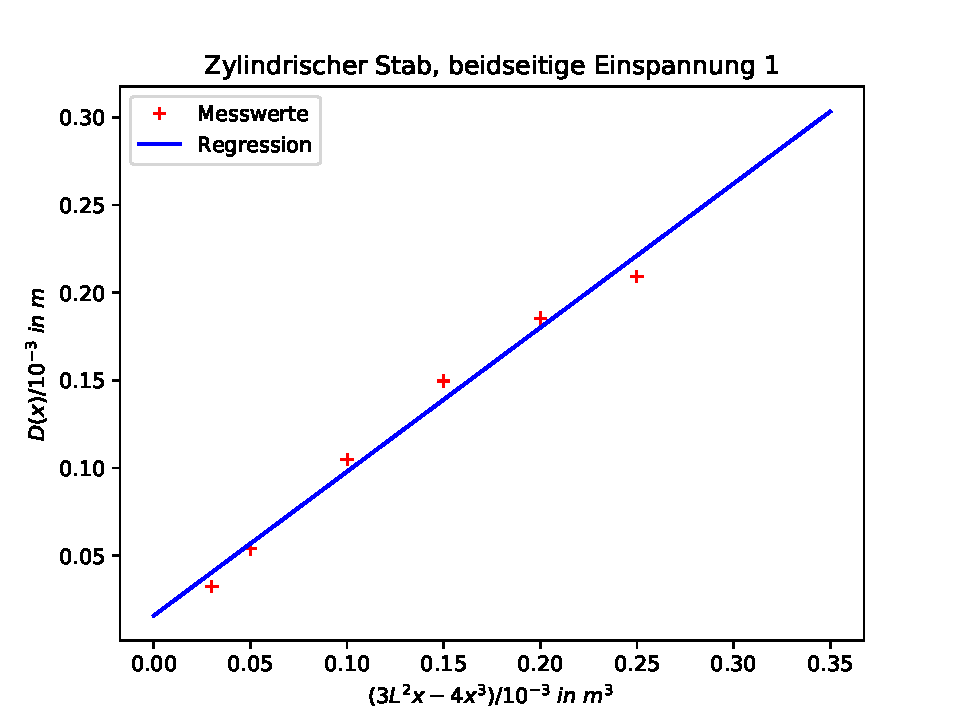
\includegraphics[width=\textwidth]{plot31.pdf}
  \caption{Zylindrischer Stab1, beidseitige Einspannung}
\end{figure}
\begin{figure}
  \centering
  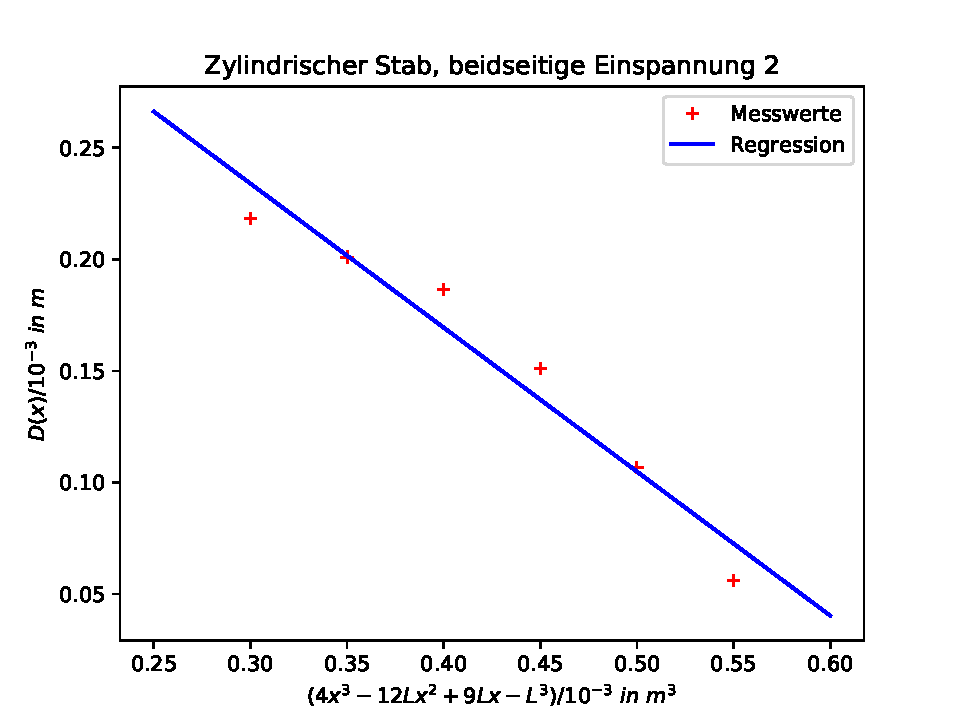
\includegraphics[width=\textwidth]{plot32.pdf}
  \caption{Zylindrischer Stab2, beidseitige Einspannung}
\end{figure}
Da das Flächenträgheitsmoment nur von $r$ abhängt, ist es gleich dem der einseitigen Einspannung.
\begin{equation*}
  I_{Zyl.} = (4,528 \pm 1,109) \cdot 10^{-10}\, \mathrm{m^4}
\end{equation*}
Das Elastizitätsmodul wird mithilfe der Formel
\begin{equation*}
  E = \frac{m \cdot g}{48 \cdot I \cdot a}
\end{equation*}
bestimmt.
Somit ergeben sich die Elastizitätsmodule
\begin{align*}
  E_1 &= (217,64 \pm 54,93) \cdot 10^6 \, \mathrm{\frac{N}{m^2}} \\
  E_2 &= (-274,56 \pm 67,32) \cdot 10^6\, \mathrm{\frac{N}{m^2}}
\end{align*}
\newpage
\subsection{Materialbestimmung}
Die Materialbestimmung erfolgt über die Bestimmung der Dichte $\rho$.
Die Formel lautet:
\begin{equation}
  \rho = \frac{m}{V}
\end{equation}
Die Masssen sind in Formel \ref{eqn:2} und \ref{eqn:9} zu finden.
Für die Bestimmung der Volumen benötigt man die Formeln
\begin{align*}
  V_{Zyl.} &= \pi \cdot {\biggl(\frac{B}{2} \biggr)}^2 \cdot L \\
  V_{R.eck} &= L \cdot B^2
\end{align*}
Somit ergeben sich die Dichten
\begin{align*}
  \rho{_{R.eck}} &=  0,2768 \cdot 10^{-4} \, \mathrm{\frac{Kg}{m^3}} \\
  \rho{_{Zyl.}} &= 0,8707 \cdot 10^{-4} \, \mathrm{\frac{Kg}{m^3}}
\end{align*}
Da die selbst errechneten $\rho$ fehlerbehaftet sind,
kann unter Berücksichtigung der Literaturwerte und der Farbe der Stäbe,
das Material des rechteckigen Stabes als  Aluminium
und das Material des zylindrischen als Messing bestimmt werden.
\\
Die Literaturwerte lauten:
\begin{align*}
\rho{_{Aluminium}} &= 2710 \, \mathrm{\frac{Kg}{m^3}}\\
\rho{_{Messing}} &= 8100 \, - \, 8700 \, \mathrm{\frac{Kg}{m^3}}
\end{align*}
\end{document}
